\documentclass[12pt]{article}

% packages
\usepackage{kantlipsum}
\usepackage[margin=1in]{geometry}
\usepackage[labelfont=it]{caption}
\usepackage[table]{xcolor}
\usepackage{subcaption,framed,colortbl,multirow}
\usepackage{amsmath,amsthm,amssymb,wasysym,mathrsfs,mathtools}
\usepackage{tikz,graphicx,pgf,pgfplots}
\usetikzlibrary{arrows, angles, quotes, decorations.pathreplacing, math, patterns, calc, positioning,shapes,backgrounds,fit}
\pgfplotsset{compat=1.16}

% custom commands
\newcommand{\N}{\mathbb{N}}
\newcommand{\Z}{\mathbb{Z}}
\newcommand{\I}{\mathbb{I}}
\newcommand{\R}{\mathbb{R}}
\newcommand{\Q}{\mathbb{Q}}
%\newcommand{\C}{\mathbb{C}}
\newcommand{\F}{\mathbb{F}}

\newcommand{\powerset}{\raisebox{.15\baselineskip}{\Large\ensuremath{\wp}}}
\DeclarePairedDelimiter{\ceil}{\lceil}{\rceil}
\DeclarePairedDelimiter\floor{\lfloor}{\rfloor}

\setlength{\fboxsep}{4pt}
\newcommand{\exercise}[2]{\section*{Exercise #1}\begin{center}\framebox{\begin{minipage}{\textwidth-10pt}#2\end{minipage}}\end{center}}
\newcommand{\problem}[2]{\section*{Problem #1}\begin{center}\framebox{\begin{minipage}{\textwidth-10pt}#2\end{minipage}}\end{center}}
\newcommand{\generic}[2]{\section*{#1}\begin{center}\framebox{\begin{minipage}{\textwidth-10pt}#2\end{minipage}}\end{center}}

\newcommand{\C}{\mathcal{C}}
\newcommand{\op}{^\text{op}}
\newcommand{\homc}{\text{Hom$_{\C}$}}


 
\begin{document}
 
\title{Homework 5\\
    \large MATH CS 120CT Category Theory}
\author{Harry Coleman}
\date{February 5, 2020}
\maketitle

\generic{}{
    Suppose $\C$ is a category and $\alpha$ is a natural transformation from the functor $\homc(-,-)$ to itself. Give a proof or counterexample: if $\alpha$ is a natural isomorphism then it is the identity.
}

If $\alpha$ is a natural isomorphism between $\homc(-,-)$ and itself, then it is not necessarily the identity. Take $\C$ to be the finitely presented category:

\begin{center}
    \begin{tikzpicture}
        \node[] (C) at (0,0) {} node[anchor=north]{$C$};
        \node[] at (3,1) {$f\circ f = id_C$};
        
        \draw[fill=black] (0,0) circle (2pt) ;
        \draw[->, thick] (C) to [out=135, in=45, looseness=20] node[above]{$f$} (C);
    \end{tikzpicture}
\end{center}
We might consider $\C$ to be the abelian group of integers modulo 2 with addition $(\Z/2, +)$, where $id_C$ is 0, $f$ is 1, and composition is addition. So the given equation $f\circ f = id_C$ might relate to the fact that $1+1=0$ in $Z/2$. Because of this, $f$ is an isomorphism on $C$, and is in fact it's own inverse. In a way, we might consider the opposite of a morphism to be it's inverse\textemdash that is, $f\op \circ f = id_C$. If this is the case, then we can say that $f=f\op$. In $Z/n$, this relates to the fact that $1$ and $-1$ are equivalent.

We now consider the functor
\[\homc(-,-): \C\op \times \C \rightarrow \textbf{Set},\]
and the category $\C\op\times\C$ (where $f\op=f$and $id_C\op=id_C$):
\begin{center}
    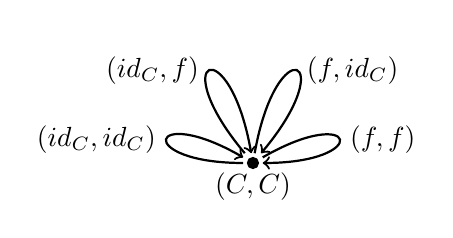
\begin{tikzpicture}
        \node[] (C) at (0,0) {} node[anchor=north]{$(C,C)$};
        
        \draw[fill=black] (0,0) circle (2pt);
        \draw[->, thick] (C) to [out=180, in=150, looseness=50] node[left]{$(id_C, id_C)$} (C);
        \draw[->, thick] (C) to [out=130, in=100, looseness=50] node[left]{$(id_C, f)$} (C);
        \draw[->, thick] (C) to [out=80, in=50, looseness=50] node[right]{$(f, id_C)$} (C);
        \draw[->, thick] (C) to [out=30, in=0, looseness=50] node[right]{$(f,f)$} (C);
    \end{tikzpicture}
\end{center}
Since $\C\op\times\C$ has only the one object $(C,C)$ and
\[\homc(-,-):(C,C)\mapsto\{id_C, f\},\]
we know that $\homc(-,-)$ maps each morphism in $\C\op\times\C$ to a function in \textbf{Set} from the set $M=\{id_C, f\}$ to itself. In other words, $M$ is the hom-set $\homc(C,C)$. There are two such functions:
\begin{alignat*}{3}
    id_M: &\quad id_C \mapsto id_C, &\quad& f \mapsto f, \\
    p: &\quad id_C \mapsto f, &\quad& f\mapsto id_C.
\end{alignat*}
The first is the identity on $M$, and the other is a permutation of its two elements. This tells us that $p\circ p = id_M$, since permuting two objects is its own inverse. We find that under $\homc(-,-)$:
\begin{alignat*}{3}
    (id_C, id_C)    &\quad\mapsto\quad id_C\circ - \circ id_C    \quad&=&\quad id_M, \\
    (id_C, f)       &\quad\mapsto\quad f\circ - \circ  id_C      \quad&=&\quad p, \\
    (f, id_C)    &\quad\mapsto\quad id_C \circ - \circ  f  \quad&=&\quad p, \\
    (f,f)        &\quad\mapsto\quad f\circ - \circ  f      \quad&=&\quad id_M.
\end{alignat*}

We now claim that $\alpha$ is a natural isomorphism in \textbf{Set} between $\homc(-,-)$ and itself if we define its one component $\alpha_{(C,C)} = p$. In order for $\alpha$ to be a natural isomorphism, we must have
\[\alpha_{(C,C)}\circ\homc(*,*) = \homc(*,*)\circ\alpha_{(C,C)},\]
for every morphism $(*,*)$ in $\C\op\times\C$. Since there is only one component $\alpha_{(C,C)}=p$ and every morphism in $\C\op\times\C$ maps to either $id_M$ or $p$ under $\homc(-,-)$, we only have to check that
\begin{align*}
    p \circ id_M &= id_M \circ p, \\
    p \circ p &= p\circ p.
\end{align*}
Since both are true, $\alpha$ is a natural transformation and, since each component of $\alpha$ is bijective in \textbf{Set}, $\alpha$ is a natural isomorphism from $\homc(-,-)$ to itself which is not the identity.










\end{document}